% 文档类:article(基础文章类),12pt(字体大小),a4paper(纸张尺寸)
\documentclass[12pt,a4paper]{article}

% ===================== 基础包引入 =====================
% 1. 中文支持(需 XeLaTeX 编译器)
\usepackage{xeCJK}
% 设置中文字体(根据本地安装字体调整,常用:SimSun/宋体、Microsoft YaHei/微软雅黑)
\setCJKmainfont{SimSun}  % 正文中文主字体
\setCJKsansfont{Microsoft YaHei}  % 中文无衬线字体(用于标题/强调)

% 2. 页面布局(边距、页眉页脚)
\usepackage{geometry}
\geometry{left=2.5cm, right=2.5cm, top=2.5cm, bottom=2.5cm}  % 统一边距

% 3. 图片插入(支持多种格式:png/jpg/pdf)
\usepackage{graphicx}
% 设置图片默认存放路径(可选,便于管理图片文件)
\graphicspath{{./images/}{./icons/}}  % 图片放在 images 和 icons 文件夹下

% 4. 表格支持(扩展表格功能,如跨列/跨行)
\usepackage{multirow}  % 跨行单元格
\usepackage{makecell}  % 单元格内换行
\usepackage{booktabs}  % 美观的表格线(替代默认三线表)

% 5. 块环境(tcolorbox:灵活的彩色/带框块)
\usepackage{tcolorbox}
% 自定义 block 环境(可按需调整颜色/字体)
\newtcolorbox{block}[1][]{  % 带可选参数的 block 环境
    colback=blue!5,    % 背景色(浅蓝色浅底)
    colframe=blue!50,  % 边框色(蓝色)
    coltext=black,     % 文字色
    fontupper=\small,  % 文字大小
    boxrule=0.8pt,     % 边框粗细
    sharp corners,     % 直角边框(可选:rounded corners 圆角)
    #1  % 接收可选参数(如自定义颜色)
}

% 6. 定理环境(amsthm:数学定理/定义/证明标准包)
\usepackage{amsthm}
% 自定义定理系列环境(编号共享,按章节递增)
\theoremstyle{plain}  % 标准定理样式(斜体)
\newtheorem{theorem}{定理}[section]  % 定理(按章节编号,如 1.1)
\newtheorem{lemma}[theorem]{引理}     % 引理(与定理共享编号)

\theoremstyle{definition}  % 定义样式(正体)
\newtheorem{definition}[theorem]{定义}  % 定义(共享编号)

\theoremstyle{remark}  % 备注样式(小字体)
\newtheorem{remark}[theorem]{备注}     % 备注(共享编号)

% 7. 数学公式(amsmath/amssymb:完整数学符号与公式支持)
\usepackage{amsmath}    % 基础数学公式(如矩阵、分式、根号)
\usepackage{amssymb}    % 扩展数学符号(如集合符号 ∀、∃、∈)

% 8. 其他辅助(目录、段落间距)
\usepackage{tocloft}    % 优化目录样式
\setlength{\parskip}{0.5em}  % 段落之间的间距(避免拥挤)


% ===================== 文档正文 =====================
\begin{document}

% 1. 标题与作者(中文标题需用 \titleCJK 包裹)
\title{\CJKfamily{Microsoft YaHei}% 标题用微软雅黑
    AI工具使用详情
}
\date{}  % 不显示日期
\maketitle

% -------------------- 第 1 章:参赛作品使用的AI工具列表 --------------------
% -------------------- 第 1 章:参赛作品使用的AI工具列表 --------------------
\section{参赛作品使用的AI工具列表}

\begin{itemize}
    \item \textbf{ChatGPT:} GPT, o4, OpenAI, 2025-09-05
    \item \textbf{Kimi:} Kimi, Latest, 月之暗面, 2025-09-05
    \item \textbf{DeepSeek:}  DeepSeek, R1 0528, 深度求索(DeepSeek), 2025-09-05
    \item \textbf{Github Copilot:} Github Copilot, GitHub, 2025-09-05
    \item \textbf{Qwen:} Qwen, 320B, 2025-09-05
    \item \textbf{Claude:} Claude, 4.0 Sonnet, Anthropic, 2025-09-05
    \item \textbf{Gemini:} Gemini, 1.5 Pro, Google DeepMind, 2025-09-05
\end{itemize}

% 根据列表建立环境
% ChatGPT Block
\newenvironment{GPTblock}
{
    \begin{tcolorbox}[colback=blue!5, colframe=blue!50, title={
        \raisebox{-.2em}{
\includegraphics[height=1.5em]{icons/openai.png}}\hspace{0.5em}\textcolor{black}{ChatGPT}
    }]
}
{
    \vspace{0.5em}
    \begin{flushright}
        \scriptsize
        \textbf{模型使用信息:} ChatGPT,GPT,o4,OpenAI,2025-09-05
    \end{flushright}
    \end{tcolorbox}
}

% Kimi Block
\newenvironment{KimiBlock}
{
    \begin{tcolorbox}[colback=purple!5, colframe=purple!50, title={
        \raisebox{-.2em}{
\includegraphics[height=1.5em]{icons/kimi-color.png}}\hspace{0.5em}\textcolor{black}{Kimi}
    }]
}
{
    \vspace{0.5em}
    \begin{flushright}
        \scriptsize
        \textbf{模型使用信息:} Kimi,Latest,月之暗面,2025-09-05
    \end{flushright}
    \end{tcolorbox}
}

% DeepSeek Block
\newenvironment{DeepSeekBlock}
{
    \begin{tcolorbox}[colback=cyan!5, colframe=cyan!50, title={
        \raisebox{-.2em}{
\includegraphics[height=1.5em]{icons/deepseek-color.png}}\hspace{0.5em}\textcolor{black}{DeepSeek}
    }]
}
{
    \vspace{0.5em}
    \begin{flushright}
        \scriptsize
        \textbf{模型使用信息:} DeepSeek,R1 0528,深度求索(DeepSeek),2025-09-05
    \end{flushright}
    \end{tcolorbox}
}

% Copilot Block
\newenvironment{CopilotBlock}
{
    \begin{tcolorbox}[colback=gray!5, colframe=gray!50, title={
        \raisebox{-.2em}{
\includegraphics[height=1.5em]{icons/githubcopilot.png}}\hspace{0.5em}\textcolor{black}{Github Copilot}
    }]
}
{
    \vspace{0.5em}
    \begin{flushright}
        \scriptsize
        \textbf{模型使用信息:} Github Copilot,GitHub,2025-09-05
    \end{flushright}
    \end{tcolorbox}
}

% Qwen Block
\newenvironment{QwenBlock}
{
    \begin{tcolorbox}[colback=yellow!5, colframe=yellow!50, title={
        \raisebox{-.2em}{
\includegraphics[height=1.5em]{icons/qwen-color.png}}\hspace{0.5em}\textcolor{black}{Qwen}
    }]
}
{
    \vspace{0.5em}
    \begin{flushright}
        \scriptsize
        \textbf{模型使用信息:} Qwen,320B,2025-09-05
    \end{flushright}
    \end{tcolorbox}
}

% Claude Block
\newenvironment{ClaudeBlock}
{
    \begin{tcolorbox}[colback=orange!5, colframe=orange!50, title={
        \raisebox{-.2em}{
\includegraphics[height=1.5em]{icons/claude-color.png}}\hspace{0.5em}\textcolor{black}{Claude}
    }]
}
{
    \vspace{0.5em}
    \begin{flushright}
        \scriptsize
        \textbf{模型使用信息:} Claude,4.0 Sonnet,Anthropic,2025-09-05
    \end{flushright}
    \end{tcolorbox}
}

% Gemini Block
\newenvironment{GeminiBlock}
{
    \begin{tcolorbox}[colback=teal!5, colframe=teal!50, title={
        \raisebox{-.2em}{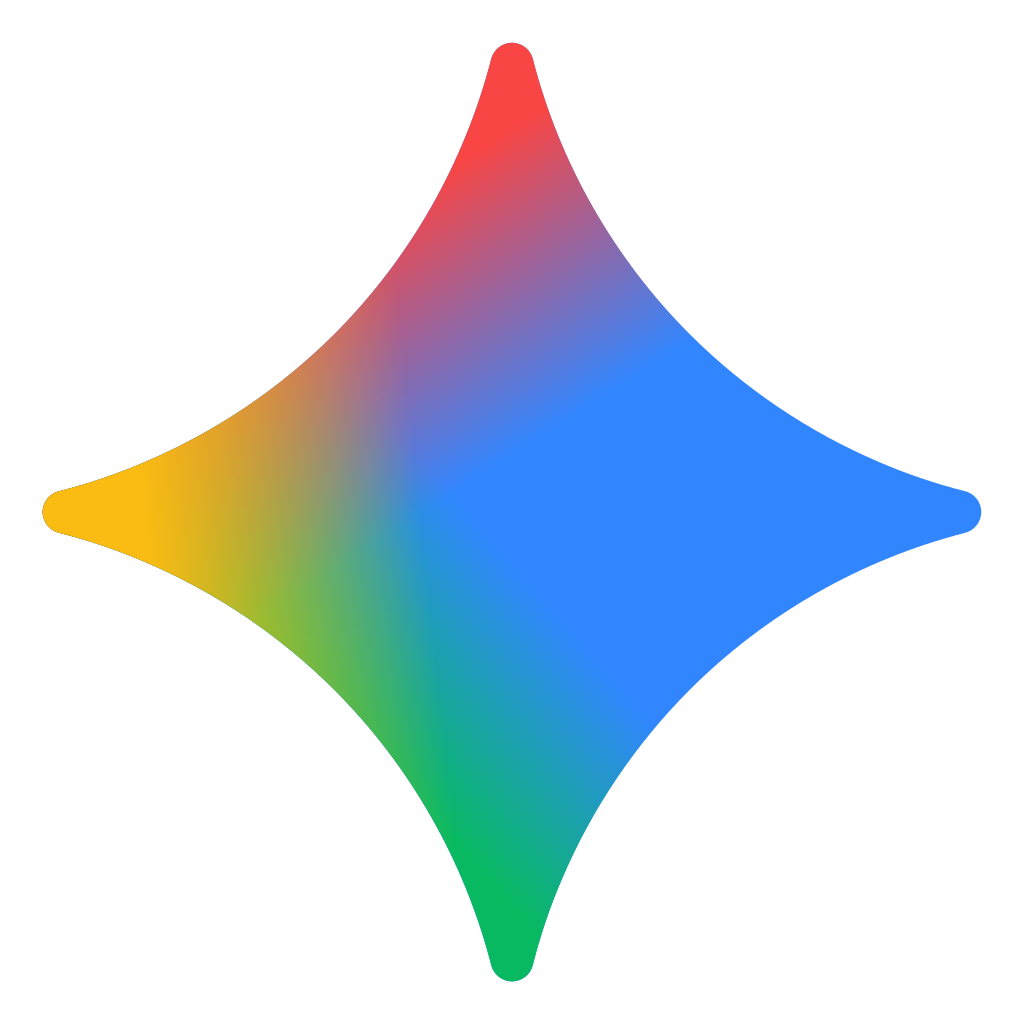
\includegraphics[height=1.5em]{icons/gemini-color.png}}\hspace{0.5em}\textcolor{black}{Gemini}
    }]
}
{
    \vspace{0.5em}
    \begin{flushright}
        \scriptsize
        \textbf{模型使用信息:} Gemini,1.5 Pro,Google DeepMind,2025-09-05
    \end{flushright}
    \end{tcolorbox}
}


\newpage

% -------------------- 第 2 章:AI 工具使用详情说明 --------------------
\section{AI 工具使用详情说明}
% 1. 用户提问 Block(浅橙色,结尾附具体使用目的和环节说明)
\begin{tcolorbox}[colback=orange!10, colframe=orange!60, title={\textcolor{black}{用户提问}}]
如何计算两个实数的和?
\vspace{0.5em}
\begin{flushright}
    \scriptsize
    \begin{flushleft}
        \textbf{具体使用目的和环节:} 本次调用 AI 工具用于解答数学基础问题,环节为“算法设计与实现”,目的是快速获得标准解法并规范表达步骤。
    \end{flushleft}
\end{flushright}
\end{tcolorbox}

% 2. AI 回答 Block 环境定义(自动带图标、标题、模型信息)
% 用法:\begin{GPTblock} ... \end{GPTblock}

% 用法示例
\begin{GPTblock}
以下是计算两数之和的简单算法:
\begin{enumerate}
    \item 输入两个实数 $x$ 和 $y$;
    \item 计算 $s = x + y$;
    \item 输出结果 $s$。
\end{enumerate}
\end{GPTblock}

% 3. 采纳和人工修改情况
\begin{tcolorbox}[colback=green!10, colframe=green!50, title={\textcolor{black}{采纳和人工修改情况}}]
\begin{itemize}
    \item \textbf{采纳情况:} AI 工具提供的解法被完全采纳。
    \item \textbf{人工修改情况:} 无需人工修改,AI 工具的解法已满足需求。
\end{itemize}
\end{tcolorbox}

% 1. 用户提问 Block(浅橙色,结尾附具体使用目的和环节说明)
\begin{tcolorbox}[colback=orange!10, colframe=orange!60, title={\textcolor{black}{用户提问}}]
如何计算两个虚数的和?
\vspace{0.5em}
\begin{flushright}
    \scriptsize
    \begin{flushleft}
        \textbf{具体使用目的和环节:} 本次调用 AI 工具用于解答数学基础问题,环节为“算法设计与实现”,目的是快速获得标准解法并规范表达步骤。
    \end{flushleft}
\end{flushright}
\end{tcolorbox}

% 2. AI 回答 Block 环境定义(自动带图标、标题、模型信息)
% 用法:\begin{geminiblock} ... \end{geminiblock}

% 用法示例
\begin{GeminiBlock}
以下是计算两数之和的简单算法:
\begin{enumerate}
    \item 输入两个虚数 $x$ 和 $y$;
    \item 计算 $s = x + y$;
    \item 输出结果 $s$。
\end{enumerate}
\end{GeminiBlock}

% 2b. 用户追问 Block(再次交互,展示追问以获取形式化结果与示例)
\begin{tcolorbox}[colback=orange!10, colframe=orange!60, title={\textcolor{black}{用户追问}}]
如果把两个虚数具体写成代数形式 $(a+bi)$ 与 $(c+di)$,其和应如何规范表示?能否再给一个带具体数字的示例来说明?
\vspace{0.5em}
\begin{flushright}
    \scriptsize
    \begin{flushleft}
        	extbf{追问目的:} 进一步明确复数加法的通式表达与数值示例,便于在论文中直接引用;仍处于“算法设计与实现”环节。
    \end{flushleft}
\end{flushright}
\end{tcolorbox}

% 2c. AI 对追问的回答
\begin{GeminiBlock}
复数(虚数是其特殊情形)加法的通式:
\[
(a+bi) + (c+di) = (a+c) + (b+d)i.
\]
其中实部相加,虚部系数相加,保持 $i$ 不变。

数值示例:
\[
(2+3i) + (1-5i) = (2+1) + (3-5)i = 3 - 2i.
\]
说明:该运算不需要额外条件,时间复杂度 $O(1)$;在实现层面可分别存储实部、虚部再组合输出。

这是一段长文本

这是一段长文本



这是一段长文本

这是一段长文本

这是一段长文本

这是一段长文本

这是一段长文本

这是一段长文本

这是一段长文本

这是一段长文本

这是一段长文本

这是一段长文本

这是一段长文本

这是一段长文本

这是一段长文本

这是一段长文本

这是一段长文本
\end{GeminiBlock}

% 3. 采纳和人工修改情况
\begin{tcolorbox}[colback=green!10, colframe=green!50, title={\textcolor{black}{采纳和人工修改情况}}]
\begin{itemize}
    \item \textbf{交互轮次:} 2(初次提问 + 1 次追问)。
    \item \textbf{采纳情况:} 初次回答与追问回答均被完全采纳。
    \item \textbf{人工修改情况:} 无需人工修改,AI 给出的通式与示例已直接满足报告中“算法说明”小节的引用需求。
\end{itemize}
\end{tcolorbox}

\end{document}